%%%%%%%%%%%%%%%%%%%%%%%%%%%%%%%%%%%%%%%%%%%%%%%%%%%%%
%                                                   %
%     Penn State Colloquium Poster Template         %
%                                                   %
% Uses Penn State Colloquium class, with options:   %
%                                                   %
% Orientation:                                      %
%     portrait (default), landscape                 %
%                                                   %
% Paper size:                                       %
%     a4paper (default), a0paper, a1paper, a2paper, %
%     a3paper, a5paper, a6paper                     %
%%%%%%%%%%%%%%%%%%%%%%%%%%%%%%%%%%%%%%%%%%%%%%%%%%%%%
\documentclass{../psuposter}
\renewcommand{\templateimagepath}{../} 


%%%%%%%%%%%%%%%%%%%%%%%%%%%%%%%%%%%%%%%%%%%%%%%%%%%%%
%               Package Dependencies                %
%%%%%%%%%%%%%%%%%%%%%%%%%%%%%%%%%%%%%%%%%%%%%%%%%%%%%
\usepackage{natbib}
\usepackage{lipsum}                                % Dummy text
\usepackage[figwidth = 0.98\linewidth]{todonotes}  % Dummy image (and more!)
\usepackage[absolute, overlay]{textpos}            % Figure placement
\usepackage{braket}
\setlength{\TPHorizModule}{\paperwidth}
\setlength{\TPVertModule}{\paperheight}
\setcitestyle{numbers,square}


%%%%%%%%%%%%%%%%%%%%%%%%%%%%%%%%%%%%%%%%%%%%%%%%%%%%%
%                 AUTHOR AND TITLE                  %
%%%%%%%%%%%%%%%%%%%%%%%%%%%%%%%%%%%%%%%%%%%%%%%%%%%%%
\title{Evolving Networks in Matter and Mind}
\author{Dani Bassett}
\institute{University of Pennsylvania}


%%%%%%%%%%%%%%%%%%%%%%%%%%%%%%%%%%%%%%%%%%%%%%%%%%%%%
%                  BEGIN DOCUMENT                   %
%%%%%%%%%%%%%%%%%%%%%%%%%%%%%%%%%%%%%%%%%%%%%%%%%%%%%
\begin{document}
\begin{frame}
\begin{columns}[t, totalwidth=\textwidth]
\begin{column}{0.45\textwidth - 1cm}


%%%%%%%%%%%%%%%%%%%%%%%%%%%%%%%%%%%%%%%%%%%%%%%%%%%%%
%                 BLOCK: BIOGRAPHY                  %
%%%%%%%%%%%%%%%%%%%%%%%%%%%%%%%%%%%%%%%%%%%%%%%%%%%%%
    \begin{block}{Speaker Biographic Summary}
    	\begin{center}
    		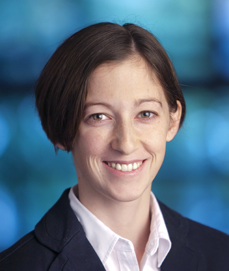
\includegraphics[width=0.68\textwidth]{images/portrait}
    	\end{center}
    	\href{https://complexsystemsupenn.com/personal}{Dr. Danielle Bassett} is the J Peter Skirkanich Professor in the Department of Bioengineering at the University of Pennsylvania, with secondary appointments in the Departments of Physics \& Astronomy, Electrical \& Systems Engineering, Neurology, and Psychiatry. She received her bachelors in physics from Penn State in 2004 and her Ph.D in physics from the University of Cambridge in 2009 respectively. She is a primary researcher in the ongoing DARPA funded Restoring Active Memory (RAM) project and has received numerous awards and honors, including  Alumni Achievement Award from the Schreyer Honors College at Penn State, APS “Rising Star” in December 2012, the Sloan Research Fellowship in 2014, a MacArthur Research Fellowship in 2014, and the Erdős–Rényi Prize for her ``fundamental contributions to our understanding of the network architecture of the human brain.''
    \end{block}


%%%%%%%%%%%%%%%%%%%%%%%%%%%%%%%%%%%%%%%%%%%%%%%%%%%%%
%            BLOCK: RESEARCH INTERESTS              %
%%%%%%%%%%%%%%%%%%%%%%%%%%%%%%%%%%%%%%%%%%%%%%%%%%%%%
    \begin{block}{Research Interests}
        Prof. Bassett’s group studies the structure and function of networks, predominantly in physical and biological systems. Her interests lie in using and developing tools and theories from complex systems science, statistical mechanics, and applied mathematics to study dynamic changes in network architecture, the interaction between topological properties of networks and physical or other constraints, and the influence of network topology on signal propagation (mechanical, electrical, informational) and system function. \cite{bassettComplexSystemsLab}
        
        \begin{center}
	    	
\includegraphics[width=0.5\textwidth]{images/research}    		
    	\end{center}
%    	\textit{Caption.} 
    	%\cite{longResearchLongLab}
    \end{block}
\end{column}
\begin{column}{0.55\textwidth - 1cm}


%%%%%%%%%%%%%%%%%%%%%%%%%%%%%%%%%%%%%%%%%%%%%%%%%%%%%
%                 BLOCK: ABSTRACT                   %
%%%%%%%%%%%%%%%%%%%%%%%%%%%%%%%%%%%%%%%%%%%%%%%%%%%%%
    \begin{block}{Talk Abstract}
    	Networks exist in both physical and conceptual spaces. Those networks can be treated as static and fixed, but in many cases evolve appreciably over a variety of time scales. In this talk, I will discuss the evolution of networks in matter and mind. I will separate my comments into three main sections. First, I will discuss principles by which to design mechanical networks that undergo precise, and pre-defined conformational changes (Kim et al. 2019 Nature Physics). Second, I will discuss connections between networks of matter and networks of mind, and relations among physical and conceptual spaces (Bassett \& Zurn, Under Contract, MIT Press). Third, I will discuss an empirical study of evolving networks of mind, as manifest in how scientists cite the work of other scientists in the reference lists of their peer-reviewed papers (Dworkin et al. 2020 Nature Neuroscience; Bertolero et al. 2020 bioRxiv), including relative imbalances in how we cite the work of gender, racial, and ethnic minorities. \cite{dworkinExtentDriversGender2020} Collectively, the work will provide a conceptual framework for understanding evolving networks in matter and mind, with important implications for our understanding of our physical world and the processes of scientific inquiry.
    \end{block}


%%%%%%%%%%%%%%%%%%%%%%%%%%%%%%%%%%%%%%%%%%%%%%%%%%%%%
%                BLOCK: BACKGROUND                  %
%%%%%%%%%%%%%%%%%%%%%%%%%%%%%%%%%%%%%%%%%%%%%%%%%%%%%
    \begin{block}{Brief Background}
    	Conformal change is an essential tool for programming and controlling the function of a wide array of mechanical systems, including robots, enzymes, and tunable metamaterials. These systems are modeled as constituent nodes, where the edges are used to impose constraints of motion, thereby producing useful coordinated motion. Prof. Bassett's group has developed fundamental mathematical principles used for designing mechanical systems capable of arbitrary infinitesimal motion or finite coordinated motion. This framework can be extended to networks with arbitrarily specifiable initial and final positions to achieve a general geometric configuration, including the creation of networks that demonstrate tristability and cooperativity.
    	\cite{kimConformationalControlMechanical2019} 
        \begin{center}
		   	
\includegraphics[width=0.75\textwidth]{images/background}    
		
		\textit{Construction and control of frames with specified outward motion} \cite{kimConformationalControlMechanical2019}
    	\end{center}
%		Second Paragraph 
		%\cite{longMorphologicalCharacterizationHVC2018} 
    \end{block}


%%%%%%%%%%%%%%%%%%%%%%%%%%%%%%%%%%%%%%%%%%%%%%%%%%%%%
%                 BLOCK: REFERENCES                 %
%%%%%%%%%%%%%%%%%%%%%%%%%%%%%%%%%%%%%%%%%%%%%%%%%%%%%
    \begin{block}{References}
        \bibliographystyle{aipnum4-1}
%        \bibliographystyle{iopart-num}
		\bibliography{references}
    \end{block}

\end{column}
\end{columns}


%%%%%%%%%%%%%%%%%%%%%%%%%%%%%%%%%%%%%%%%%%%%%%%%%%%%%
%                    FOOTER TEXT                    %
%%%%%%%%%%%%%%%%%%%%%%%%%%%%%%%%%%%%%%%%%%%%%%%%%%%%%
\begin{textblock}{0.5}(0.18, 0.94)
    \color{white}
    \sffamily
    \textbf{Eberly College of Science}
    \\
    Department of Physics
\end{textblock}


%%%%%%%%%%%%%%%%%%%%%%%%%%%%%%%%%%%%%%%%%%%%%%%%%%%%%
%                   END TEMPLATE                    %
%%%%%%%%%%%%%%%%%%%%%%%%%%%%%%%%%%%%%%%%%%%%%%%%%%%%%
\end{frame}
\end{document}
